% documentclass
% set font size=11 (11pt)
% set paper format=A4 (a4paper)
% set equation alignment to left (fleqn)
\documentclass[11pt,a4paper,fleqn]{article}


% Preamble
% use the inputenc and fontenc packages to use French accents
\usepackage[utf8]{inputenc}
\usepackage[T1]{fontenc}
% allow for arbitrary font size
\usepackage{anyfontsize}
% set the font as Time New Roman (the Latex equivalent, at least)
% \usepackage{mathptmx}
% set the size of the document margins using the geometry package
\usepackage[lmargin=0.97in,rmargin=0.97in,tmargin=1.4in,bmargin=1.4in]{geometry}
% turn the color of footnote markers to black
\renewcommand\thefootnote{\textcolor{black}{\arabic{footnote}}}
% suppress indents on footnotes
\usepackage[hang,flushmargin]{footmisc}
% automatically generates colored brackets around references
\usepackage{fncylab} \labelformat{equation}{(#1)}
% supress indent on new paragraphs
\setlength{\parindent}{0pt}
% use the amsmath package to include mathematical symbols
\usepackage{amsmath}
% suppress the space between the left margin and the equations (fleqn still leaves some space by default)
\setlength{\mathindent}{0pt}
% create a new environment to left flush the equation with the align environment
\makeatletter
\newenvironment{lflalign}{ \vspace{-3mm}%
  \def\align@preamble{%
    &\strut@
    \setboxz@h{\@lign$\m@th\displaystyle{####}$}%
    \ifmeasuring@\savefieldlength@\fi
    \set@field
    \hfil
    \tabskip\z@skip
    &\setboxz@h{\@lign$\m@th\displaystyle{{}####}$}%
    \ifmeasuring@\savefieldlength@\fi
    \set@field
    \hfil
    \tabskip\alignsep@
  }
  \flalign}
{\endflalign}
\makeatother
% use the ammssymb package to use mathematical symbols
\usepackage{amssymb}
% create new commands for mathematical symbols
\DeclareMathOperator{\N}{\mathbb{N}}
\DeclareMathOperator{\Z}{\mathbb{Z}}
\DeclareMathOperator{\Q}{\mathbb{Q}}
\DeclareMathOperator{\R}{\mathbb{R}}
\DeclareMathOperator{\Pb}{\mathbb{P}}
% declare the cmsy (computer modern symbol) math alphabet to define appropriate fonts for the U and N mathematical symbols
\DeclareMathAlphabet\mathbcal{OMS}{cmsy}{m}{n}
% create new commands for mathematical symbols
\DeclareMathOperator{\E}{\mathbcal{E}}
\DeclareMathOperator{\Ex}{\mathbb{E}}
\DeclareMathOperator{\F}{\mathbcal{F}}
\DeclareMathOperator{\G}{\mathbcal{G}}
\DeclareMathOperator{\M}{\mathbcal{M}}
\DeclareMathOperator{\HH}{\mathbcal{H}}
\DeclareMathOperator{\QQ}{\mathbcal{Q}}
\DeclareMathOperator{\PP}{\mathbcal{P}}
\DeclareMathOperator{\Noo}{\mathbcal{N}}
\DeclareMathOperator{\U}{\mathbcal{U}}
% use the bbm package to be able to use the double stroke 1 for the indicator function
\usepackage{bbm}
\DeclareMathOperator{\ind}{\mathbbmss{1}}
% use the bm package to use bold characters in math mode
\usepackage{bm}
% create a new command for black square bullets
\newcommand{\bs}{\scalebox{0.7}{$\blacksquare$} \hspace{2mm}}
% use the relsize package to be abe to change the size of mathematical symbols
\usepackage{relsize}
% define a new command for in-line small summation
\newcommand{\ssumm}[2]{\underset{\scriptscriptstyle #1}{\overset{\scriptscriptstyle #2}{\mathlarger{\mathlarger{\mathlarger{\Sigma}}}}} \hspace{0.5mm}}
% define a new command for in-line small products
\newcommand{\sprod}[2]{\underset{\scriptscriptstyle #1}{\overset{\scriptscriptstyle #2}{\mathlarger{\mathlarger{\mathlarger{\Pi}}}}} \hspace{0.5mm}}
% Use the caption package to customize captions (titles) of tables and graphs
\usepackage[font=small,labelfont=bf]{caption}
% use float package to force figure the be positioned where indicated
\usepackage{float}
% use the graphicx package to be able to resize tables
\usepackage{graphicx}


\begin{document}

% command to check unused bibliography entries
% \nocite{*}

\begin{center}
{\fontsize{15pt}{22pt}\selectfont \textbf{Proposition de correction pour le quizz de statistiques} \par}
\end{center}

\vspace{5mm}

{\fontsize{12pt}{22pt} \textbf{1. Général:}\par}

\vspace{5mm}

1) Que vaut $Cov(X+\mu)$ pour tout $\mu \in \R^p$ déterministe, et tout vecteur aléatoire $X \in \R^p$? \vspace{2mm}

On a:
\begin{lflalign}
& \ Cov(X+\mu) \nonumber \\
= \ & \ \Ex \left[ \left(X+\mu-\Ex(X+\mu) \right) \left(X+\mu-\Ex(X+\mu) \right)^T \right] \nonumber \\
= \ & \ \Ex \left[ \left(X+\mu-\Ex(X)-\mu \right) \left(X+\mu-\Ex(X)-\mu \right)^T \right] \nonumber \\
= \ & \ \Ex \left[ \left(X-\Ex(X) \right) \left(X-\Ex(X) \right)^T \right] \nonumber \\
= \ & \ Cov(X) \nonumber
\end{lflalign} \vspace{1mm}

2) Que vaut $Cov(AX)$, pour toute matrice $A \in \R^{m \times p} $ et tout vecteur aléatoire $X \in \R^p$? \vspace{2mm}

On a:
\begin{lflalign}
\ & \ Cov(AX) \nonumber \\
= \ & \ \Ex \left[ \left(AX-\Ex(AX) \right) \left(AX-\Ex(AX) \right)^T \right] \nonumber \\
= \ & \ \Ex \left[ \left(AX-A\Ex(X) \right) \left(AX-A\Ex(X) \right)^T \right] \nonumber \\
= \ & \ \Ex \left[ \left(A[X-\Ex(X)] \right) \left(A[X-\Ex(X)] \right)^T \right] \nonumber \\
= \ & \ \Ex \left[ A \left([X-\Ex(X)] \right) \left([X-\Ex(X)] \right)^T A^T \right] \nonumber \\
= \ & \ A \Ex \left[ (X-\Ex(X)) (X-\Ex(X))^T \right] A^T \nonumber \\
= \ & \ A \ Cov(X) \ A^T \nonumber
\end{lflalign} \vspace{1mm}

3) Donner un modèle naturel pour ``un lancer de dé'' (non-nécessairement équilibré)? \vspace{2mm}

Un modèle naturel (ou famille de loi naturelle) pour ``un lancer de dé'' est la distribution catégorielle ou multi-Bernoulli, qui généralise la loi Bernoulli à $k$ catégories. Ici, on aura $k=6$, et $\M=\{ \Pb_\theta: \theta \in \R^6 , \ssumm{i=1}{6} \theta_i=1 \}$. \vspace{5mm}

4) Soit $x_1, x_2, \hdots, x_n$ i.i.d. tel que $\Ex [x_1^2]<\infty$. Quel estimateur $\hat{\mu}$ minimise $\ssumm{}{}_{i=1}^n(x_i-\mu)^2$? \\ Donner son biais et sa variance, pour tout $n>1$. \vspace{2mm}

On cherche: $\hat{\mu}=\underset{\mu}{argmin} \ \ssumm{i=1}{n} (x_i-\mu)^2$. La condition de premier ordre est:
\begin{lflalign}
& \ \frac{d}{d \mu} \left(\ssumm{i=1}{n} (x_i-\mu)^2\right)=0 \nonumber \\
\Leftrightarrow \ & \ -2 \ssumm{i=1}{n} (x_i-\mu)=0 \nonumber \\
\Leftrightarrow \ & \ \ssumm{i=1}{n} (x_i-\mu)=0 \nonumber \\
\Leftrightarrow \ & \ \ssumm{i=1}{n} x_i=n \mu \nonumber \\
\Leftrightarrow \ & \ \mu = \frac{1}{n} \ssumm{i=1}{n} \ x_i \nonumber
\end{lflalign}

L'estimateur est donc $\hat{\mu}=\frac{1}{n} \ssumm{i=1}{n} \ x_i$. Son biais est donné par:
\begin{lflalign}
& \ Biais(\hat{\mu}, \mu) \nonumber \\
= \ & \ \Ex_\theta (\hat{\mu}-\mu) \nonumber \\
= \ & \ \Ex_\theta \left( \frac{1}{n} \ \ssumm{i=1}{n} x_i-\mu \right) \nonumber \\
= \ & \ \frac{1}{n} \ \ssumm{i=1}{n} \Ex_\theta (x_i)-\mu \nonumber \\
= \ & \ \frac{1}{n} \ n \Ex_\theta (X)-\mu \hspace{5mm} \text{(car les } x_i \text{ sont identiquement distribuées)} \nonumber \\
= \ & \ \Ex_\theta (X)-\mu \nonumber \\
= \ & \ \mu-\mu \nonumber \\
= \ & \ 0 \nonumber
\end{lflalign}

Sa variance est donnée par:
\begin{lflalign}
& \ var(\hat{\mu}) \nonumber \\
= \ & \ var \left( \frac{1}{n} \ssumm{i=1}{n} x_i \right) \nonumber \\
= \ & \ \frac{1}{n^2} var \left( \ssumm{i=1}{n} x_i \right) \nonumber \\
= \ & \ \frac{1}{n^2} \ \ssumm{i=1}{n} var (x_i) \hspace{5mm} \text{(par indépendence des } x_i \text{)} \nonumber \\
= \ & \ \frac{1}{n^2} \ n \ var (X) \hspace{5mm} \text{(car les } x_i \text{ sont identiquement distribuées)} \nonumber \\
= \ & \ \frac{1}{n} \ var (X) \nonumber
\end{lflalign}

\pagebreak

5) Que vaut le biais de $\frac{1}{n} \ssumm{i=1}{n} (y_i-\bar{y}_n)^2$ ($\bar{y}_n$ est la moyenne empirique) pour des $y_i$ i.i.d. gaussiens, centrés et de variance $\sigma^2$? \vspace{2mm}

On définit la variance empirique comme $\tilde{\sigma}^2=\frac{1}{n} \ssumm{i=1}{n} (y_i-\bar{y}_n)^2$. On peut ensuite la manipuler pour obtenir:
\begin{equation}
\tilde{\sigma}^2=\frac{1}{n} \ssumm{i=1}{n} (y_i-\bar{y}_n)^2 \hspace{3mm} \Leftrightarrow \hspace{3mm} \frac{n}{\sigma^2} \tilde{\sigma}^2 = \ssumm{i=1}{n} \frac{(y_i-\bar{y}_n)}{\sigma^2}^2
\nonumber \end{equation}
Il découle ensuite du théorème de Cochran que:
\begin{equation}
\ssumm{i=1}{n} \frac{(y_i-\bar{y}_n)}{\sigma^2}^2 \sim \chi^2(n-1) \hspace{3mm} \Leftrightarrow \hspace{3mm}  \frac{n}{\sigma^2} \tilde{\sigma}^2 \sim \chi^2(n-1)
\nonumber \end{equation}
Les propriétés de la distribution $\chi^2$ impliquent que $\frac{n}{\sigma^2} \tilde{\sigma}^2$ a une espérance de $(n-1)$ et une variance de $2(n-1)$. On conclut alors:
\begin{equation}
\Ex(\frac{n}{\sigma^2} \tilde{\sigma}^2)=n-1 \ \Leftrightarrow \ \Ex(\tilde{\sigma}^2)=\frac{n-1}{n} \sigma^2
\nonumber \end{equation}
Le biais est donc de:
\begin{equation}
Biais(\tilde{\sigma}^2, \sigma^2)=\Ex(\tilde{\sigma}^2)-\sigma^2=\frac{n-1}{n} \sigma^2-\sigma^2=-\frac{1}{n}\sigma^2
\nonumber \end{equation} \vspace{1mm}

6) On suppose que l'on observe $y_1, \hdots, y_n$, des variables réelles i.i.d., gaussiennes, centrées et de variance $\sigma^2$. Quel est le risque quadratique de l'estimateur $\frac{1}{n} \ssumm{i=1}{n} (y_i-\bar{y}_n)^2$ de $\sigma^2$ ($\bar{y}_n$ est la moyenne empirique)?  \vspace{2mm}

On utilise le même raisonnement qu'à la question précédente, qu'on complète en ajoutant que:
\begin{equation}
var(\frac{n}{\sigma^2} \tilde{\sigma}^2)=2(n-1) \ \Leftrightarrow \ \frac{n^2}{\sigma^4} var(\tilde{\sigma}^2)=2(n-1) \ \Leftrightarrow \ var(\tilde{\sigma}^2) = \frac{2\sigma^4(n-1)}{n^2}
\nonumber \end{equation}
On utilise alors la définition du risque quadratique pour obtenir: \vspace{2mm}
\begin{lflalign}
& \ R(\tilde{\sigma}^2) \nonumber \\
= \ & \ var(\tilde{\sigma}^2)+(biais(\tilde{\sigma}^2))^2 \nonumber \\
= \ & \ \frac{2\sigma^4(n-1)}{n^2}+\frac{\sigma^4}{n^2} \nonumber \\
= \ & \ \frac{\sigma^4(2n-1)}{n^2} \nonumber
\end{lflalign} \vspace{2mm}

7) Quelle est la projection orthogonale du vecteur $\bm{y} \in \R^n$ sur Vect($1_n$), avec $1_n=(1,\hdots,1)^T \in \R^n$? \vspace{2mm}

Soit $\bm{y} \in \R^n$ et $\bm{v}=1_n=(1,\hdots,1)^T \in \R^n$. On considère la projection orthogonale $\bm{w}$ de $\bm{y}$ sur $\bm{v}$, que l'on peut représenter par le grahique suivant:

\begin{figure}[H] \begin{center}
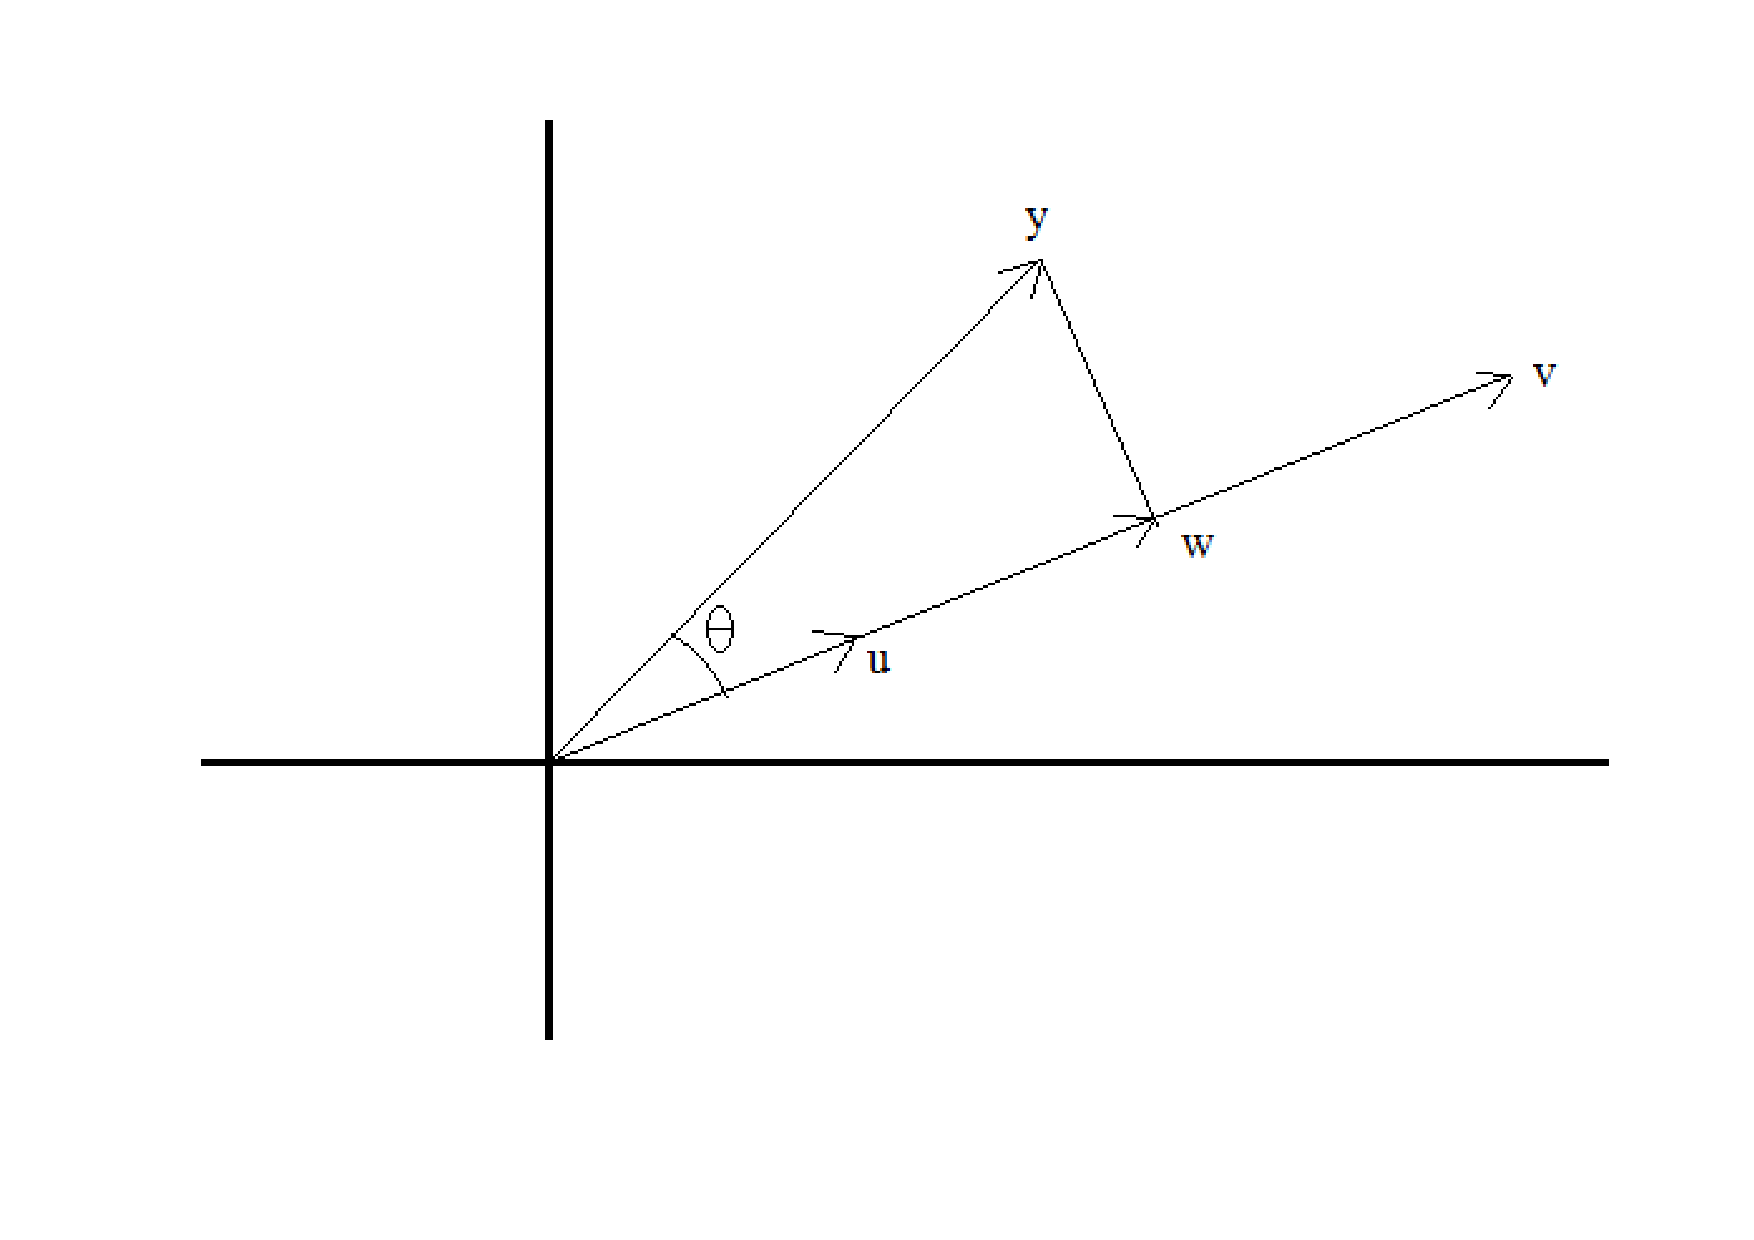
\includegraphics[scale=0.4]{images/graph1.pdf} \vspace{-3mm}
\end{center} \end{figure}

Le vecteur $\bm{u}$ est un vecteur unitaire dans la direction de $\bm{w}$ tel que $u=\frac{1}{\sqrt{n}} 1_n$. On note que par construction $\bm{w}= \|w\| \bm{u}$. Par definition de la fonction cosinus, on a également $cos(\theta)=\frac{\|w\|}{\|y\|}$ et par définition du produit scalaire on a $cos(\theta)=\frac{\langle u,y \rangle}{\|u\| \|y\|}$. En combinant ces deux dernières expressions, on obtient $\|w\|=\langle u,y \rangle $. En substituant dans la première expression, on obtient $w=\langle u,y \rangle \ u$ et donc:
\begin{lflalign}
& \ w \nonumber \\
= \ & \ \langle u,y \rangle \ u \nonumber \\
= \ & \ \langle \frac{1}{\sqrt{n}} 1_n,y \rangle \ \frac{1}{\sqrt{n}} 1_n \nonumber \\
= \ & \ \frac{1}{n} \langle 1_n,y \rangle \ 1_n \nonumber \\
= \ & \ \frac{1}{n} \ (\ssumm{i=1}{n} y_i) \ 1_n \nonumber \\
= \ & \ \bar{y} \ 1_n \nonumber \\
= \ & \ \left( \begin{matrix} \bar{y} \\ \bar{y} \\ \vdots \\ \bar{y} \end{matrix} \right) \nonumber
\end{lflalign} \vspace{2mm}

8) Quels sont les vecteurs $\bm{y} \in \R^n$ tels que $var_n(\bm{y})=0$ ($var_n$ est la variance empirique)?

On obtient que $var_n(\bm{y})=0$ si et seulement si $\frac{1}{n} \ssumm{i=1}{n} (y_i-\bar{y}_n)^2=0$. Celà implique que $y_i=\bar{y} \ \forall i$ (car sinon il existe un $i$ tel que $(y_i-\bar{y}_n)^2>0$ et donc $\ssumm{i=1}{n} (y_i-\bar{y}_n)^2>0$), ce qui n'est possible que si $y_1=y_2=\hdots=y_n=y$, pour $y$ un scalaire donné. On conclut donc que ces vecteurs sont de la forme $\bm{y}=y . 1_n$.













\vspace{5mm}

{\fontsize{12pt}{22pt} \textbf{2. Moindres carrés unidimensionnels:}\par}

\vspace{5mm}

On observe $\bm{y}=(y_1, \hdots, y_n)^T$ et $\bm{x}=(x_1, \hdots, x_n)^T$.

1) La fonction $(\theta_0, \theta_1)\rightarrow \frac{1}{2} \ssumm{}{}_{i=1}^n (y_i-\theta_0-\theta_1 x_i)^2$ est-elle convexe ou concave?  \vspace{2mm}

On considère la fonction $f=(y_i-\theta_0-\theta_1 x_i)^2$. Pour estimer sa convexité, on calcule sa Hessienne: \\
\begin{lflalign}
\ & \ \frac{\partial f}{\partial \theta_0} = -2 (y_i-\theta_0-\theta_1 x_i) \nonumber \\
\ & \ \frac{\partial^2 f}{\partial \theta_0^2} = 2 \nonumber \\
\ & \ \frac{\partial f}{\partial \theta_1} = -2 x_i (y_i-\theta_0-\theta_1 x_i) \nonumber \\
\ & \ \frac{\partial^2 f}{\partial \theta_1^2} = 2 x_i^2 \nonumber \\
\ & \ \frac{\partial^2 f}{\partial \theta_1 \partial \theta_2} = 2 x_i \nonumber 
\end{lflalign} 

La Hessienne $H$ est donc donnée par $H=\left( \begin{matrix} 2 & 2 x_i \\ 2 x_i & 2 x_i^2 \end{matrix} \right)$. On note que la matrice est singulière (sa seconde colonne est la première multipliée par $x_i$), donc au moins une de ses valeurs propres est 0. En utilisant le fait que la trace est la somme des valeurs propres, on obtient que la seconde valeur propre est $2(1+x_i^2)$, qui est toujours positive. Donc la Hessienne $H$ est symétrique semi-définie positive, et la function $f$ est convexe. Comme la fonction $(\theta_0, \theta_1)\rightarrow \frac{1}{2} \ssumm{}{}_{i=1}^n (y_i-\theta_0-\theta_1 x_i)^2$ est une somme de fonctions convexes, elle est convexe elle-même.

\vspace{5mm}

{\fontsize{12pt}{22pt} \textbf{3. Moindres carrés:}\par}

\vspace{5mm}

1) Ecrire un pseudo-code de descente de gradient pour résoudre le problème des moindres carrés.  \vspace{2mm}
\underline{Initialisation} \\
$(\theta_0^0, \theta_1^0)$: valeurs initiales de $\theta$ \\
$T$: nombre maximum d'itérations \\
$\varepsilon$: critère d'arrêt \\
$\alpha$: pas de l'algorithme \\

\underline{Boucle} \\
for $1 \leq t \leq T$: \\ \\
\phantom{a} \hspace{4mm} $(\theta_0^{t+1}, \theta_1^{t+1}) := (\theta_0^{t+1}, \theta_1^{t+1}) - \alpha . \nabla f(\theta_0^{t}, \theta_1^{t})$ \\
\phantom{a} \hspace{4mm} avec (selon le cours) $\nabla f(\theta_0^{t}, \theta_1^{t}) = X^T (X \theta - Y)$ \\ \\
\phantom{a} \hspace{4mm} soit (en utilisant la fonction de la question 2.2): \\
\phantom{a} \hspace{4mm} $\theta_0^{t+1} := \theta_0^t + \alpha \ssumm{i=1}{n} (y_i - \theta_0 - \theta_1 x_i)$ \\
\phantom{a} \hspace{4mm} $\theta_1^{t+1} := \theta_1^t + \alpha \ssumm{i=1}{n} x_i (y_i - \theta_0 - \theta_1 x_i)$ \\ \\
\phantom{a} \hspace{4mm} Stop si critère inférieur à $\varepsilon$ \\ \\
Fin de la boucle \\ \\
Return $(\theta_0^T, \theta_1^T)$ \\

Critères d'arrêt possibles: \\
$\| \nabla f(\theta_0^{t}, \theta_1^{t}) \| \leq \varepsilon$ \\
$| f(\theta_0^{t+1}, \theta_1^{t+1}) - f(\theta_0^{t}, \theta_1^{t}) | \leq \varepsilon$ \\
$ \| \theta^{t+1} - \theta^{t} \| \leq \varepsilon$ \hspace{5mm} avec $\theta = (\theta_0, \theta_1)$ \\
$ \frac{\| \theta^{t+1} - \theta^{t} \|}{\| \theta^{t} \|} \leq \varepsilon$ \hspace{5mm} avec $\theta = (\theta_0, \theta_1)$
\vspace{5mm}


10)  On suppose que X est de rang plein et on note $\hat{\theta}$ l’estimateur OLS. On note $\tilde{X}=(X_1,\hdots,X_p)$.On change l’échelle d’une des variables: $X_k$ est remplacé par $X_k b$, où $b>0$. \\
a) Soit $X_b=(1, X_1,\hdots, X_k b, \hdots, X_p)$. Montrer que $X_b = X D$ où $D$ est une matrice diagonale que l’on précisera. \\
On utilise simplement la définition de $X_b$ pour obtenir: \\
$X_b
= \left( \begin{matrix} 1 & X_1 & \hdots & X_k b & \hdots & X_p \end{matrix} \right)
= \left( \begin{matrix} 1 \times 1 & 1 \times X_1 & \hdots & b \times X_k & \hdots & 1 \times X_p \end{matrix} \right)$ \\
$ \left( \begin{matrix} 1 & X_1 & \hdots & X_k & \hdots & X_p \end{matrix} \right) \times
\left( \begin{matrix} 1 & & & & & \\ & 1 & & & & \\ & & \ddots & & & \\ & & & b & & \\ & & & & \ddots & \\ & & & & & 1 \end{matrix} \right)
= X D$ \\ \\
$D$ est donc la matrice identité de dimension $p+1$ dont l'entrée diagonale $k+1$ est remplacée par $b$. \\
b)  Soit $\hat{\theta}_{b,n}$ l’estimateur OLS associé à $X_b$. Exprimer $\hat{\theta}_{b,n}$ en fonction de $\hat{\theta}_{n}$ et de $D$. \\
Par les équations normales, l'estimateur OLS $\hat{\theta}_{b,n}$ est égal à: \\
$\hat{\theta}_{b,n}
=(X_b^T X_b)^{-1}(X_b^T y)
=[(X D)^T (X D)]^{-1}[(X D)^T y]
=[D^T X^T X D]^{-1}[D^T X^T y]$ \\
$=[D^{-1} (X^T X)^{-1} (D^T)^{-1}] \ [D^T X^T y]
=D^{-1} (X^T X)^{-1} X^T y
=D^{-1} \hat{\theta}_{n}$ \\
Autrement dit, l'estimateur $\hat{\theta}_{b,n}$ est égal à l'estimateur $\hat{\theta}_{n}$ dont le coefficient $k+1$ a été multiplié par $1/b$. \\
c) Donner la variance de $\hat{\theta}_{b,n}$. \\
On utilise simplement les propriétés de la variance (et le fait que $D$ est diagonale) pour obtenir: \\
$Var(\hat{\theta}_{b,n})=Var(D^{-1} \hat{\theta}_{n})=(D^{-1})^2 Var(\hat{\theta}_{n})=\sigma^2 (D^{-1})^2 (X^T X)^{-1}$ \\
d) La prédiction donnée par le modèle est: \\
$\hat{y}_b
=X_b \hat{\theta}_{b,n}
=(X D) (D^{-1} \hat{\theta}_{n})
=X \hat{\theta}_{n}
=\hat{y}$ \\
Autrement dit, la prédiction n'est elle pas affectée par le changement d'échelle d'une des variables. \vspace{2mm}

11) Donner une formule explicite du problème $argmin_\theta \ \frac{1}{2} (y-X \theta)^T \Omega (y-X \theta)$ pour une matrice $\Omega=diag(w_1, \hdots, w_n)$ définie positive, dans le cas où $X$ est de plein rang. \\
On commence par développer la forme quadratique: \\
$\frac{1}{2} (y-X \theta)^T \Omega (y-X \theta)
=\frac{1}{2} \left[ y^T \Omega y + \theta^T X^T \Omega X \theta - 2 \theta^T X^T \Omega y \right]$ \\
(où pour obtenir le terme $2 \theta^T X^T \Omega y$ on a utilisé le fait qu'un scalaire est égal à sa transposée, et que $\Omega$ est symétrique). \\
Pour trouver l'argmin, on utilisera les règles suivantes de dérivées matricielles:\\
- Si $a$ et $b$ sont des vecteurs, on a: $\frac{\partial b^T a}{\partial b} = a$. Cela implique que: $\frac{\partial 2 \theta^T X^T \Omega y}{\partial \theta} = 2 X^T \Omega y$. \\
- Si $A$ est une matrice symétrique et $b$ un vecteur, on a: $\frac{\partial b^T A b}{\partial b} = 2 A b$. Cela implique que: $\frac{\partial \theta^T X^T \Omega X \theta}{\partial \theta} = 2 X^T \Omega X \theta$. \\
On conclut que:
\begin{lflalign}
& \ \frac{\partial }{\partial \theta}\left( \ \frac{1}{2} (y-X \theta)^T \Omega (y-X \theta) \right)=0 \nonumber \\
\Leftrightarrow \ & \ \frac{\partial }{\partial \theta} \left( \frac{1}{2} \left[ y^T \Omega y + \theta^T X^T \Omega X \theta - 2 \theta^T X^T \Omega y \right] \right)=0 \nonumber \\
\Leftrightarrow \ & \ \frac{1}{2} \left( 2 X^T \Omega y - 2 X^T \Omega X \theta \right) = 0 \nonumber \\
\Leftrightarrow \ & \ X^T \Omega y - X^T \Omega X \theta = 0 \nonumber \\
\Leftrightarrow \ & \ X^T \Omega X \theta = X^T \Omega y \nonumber \\
\Leftrightarrow \ & \  \hat{\theta} = (X^T \Omega X)^{-1} (X^T \Omega y) \nonumber
\end{lflalign}




\bigskip
\bigskip

\textbf{12). Dans le cas du mod\'ele de régression avec désign aléatoire, décrire l'asymptotique de l'estimateur des moindre carr\'ees. On donnera la loi asymptotique de $\sqrt{n} (\hat \beta - \beta^{*})$.}

\bigskip

(Le mod\'ele \textit{Random Design} n'a pas \'et\'e trait\'e en cours. En revanche, une question sur la loi asymptotique avec le mod\'ele gaussien peut tomber).

\bigskip

\begin{itemize}
	\item \textit{Mod\'ele gaussien}
\end{itemize}

Pour \'etudier la convergence de $\hat \beta$, on fait appel au th\'eor\`eme central limite (TCL). On se base sur le calcul du biais $\hat \beta$ :

$$ \hat \beta - \beta^{*} = (X^T X)^{-1} X^T \varepsilon $$

$\hat \beta - \beta^{*}$ est une combinaison lin\'eaire certaine de lois ind\'ependantes $\varepsilon_i$ ce qui permet d'appliquer le TCL (condition 1).

\bigskip

Pour la variance, on suppose que l'hypoth\`ese suivante est v\'erifi\'e avec $V_X$ une matrice finie definie-positive (les variables explicatives conservent de la variance quand $n \rightarrow +\infty$, soit plus d'observations apportent plus d'information ce qui exclut la possibilit\'e d'une multicolin\'earit\'e stricte au niveau asymptotique) :

$$ \lim_{n\rightarrow +\infty} \frac{1}{n}(X^T X)^{-1} = V_X $$

D'où (condition 2) :

$$ \lim_{n\rightarrow +\infty} \mathbf{V}(\sqrt{n} (\hat \beta - \beta^{*})) = \lim_{n\rightarrow +\infty} n \sigma^2 (X^T X)^{-1} = \lim_{n\rightarrow +\infty} \sigma^2 \Bigl(\frac{X^T X}{n}\Bigl)^{-1} = \sigma^2 V_X^{-1} $$

\bigskip

Cons\'equence, en partant du r\'esultat que :

$$ \sqrt{n} (\beta - \beta^{*}) \sim \mathcal{N}(0, \sigma (X^T X)^{-1} ) $$

\bigskip

On d\'eduit que $\beta - \beta^{*}$ converge en loi vers :

$$ \sqrt{n} (\beta - \beta^{*}) \rightarrow  \mathcal{N}(0, \sigma V_X^{-1} )$$

\bigskip

\begin{itemize}
	\item \textit{Mod\'ele d\'esign al\'eatoire}
\end{itemize}

(Hors programme)

\bigskip
\bigskip

\textbf{13) Dans le cas du mod\'ele de r\'egression avec design d\'eterministe et bruit gaussien centr\'e de variance $\sigma^2$, donner la loi de l'estimateur des moindre carr\'ees $\hat \beta$.}

\bigskip

Dans le mod\'ele gaussien, les perturbations (ou le bruit blanc) $(\varepsilon_i)_{i=1,...,n}$ sont des variables aléatoires réelles gaussiennes telles que : $ \varepsilon_i \sim^{i.i.d} \mathcal{N}(0,\sigma^2)$ et en forme vectorielle $ \varepsilon \sim^{i.i.d} \mathcal{N}(0,\sigma^2 I_n)$.

\bigskip

Or les variables à expliquer $Y$ suivent aussi une loi gaussienne puisque $Y = X\beta^{*} + \varepsilon$ est une combinaison linéaire additive de variables al\'eatoires gaussiennes. D'où : $Y_i \sim \mathcal{N}(X_i^T\beta^{*},\sigma^2)$.

\bigskip

$\hat \beta$ est une combinaison lin\'eaire certaine des $Y_i$, d'où à l'instar de $Y$, le vecteur $\hat \beta$ suit aussi une loi normale d'esp\'erance $\mu$ et de variance-covariance $\Sigma$. Le calcul du biais et de la variance de l'estimateur $\hat \beta$ nous donne ces 2 quantit\'es :

$$ \mathbf{E}(\hat \beta) = \beta^{*} \qquad \mathbf{V}(\hat \beta) = \sigma^2 (X^T X)^{-1}$$

Ainsi :

$$ \hat \beta \sim \mathcal{N}(\beta^{*},\sigma^2 (X^T X)^{-1}) $$

Et en particulier :

$$ j = 1,...,p \qquad \hat \beta_{j} \sim \mathcal{N}(\beta_j^{*},\sigma^2 (X^T X)^{-1}_{j,j}) $$

\bigskip
\bigskip







\vspace{5mm}

14) Dans le cas du modèle de régression avec design déterministe où X est de plein rang p, donner la valeur du risque de prédiction. \\

$$ Rpred(\hat{\theta}_n) = E\left[\| Y^* - \hat{Y} \|^2_2\right] $$
$$ Rpred(\hat{\theta}_n)  = E\left[\| X(\hat{\theta}_n - \theta^*) \|^2_2\right] $$
$$ Rpred(\hat{\theta}_n) = E \left[ \| X(X^TX)^{-1}X^T \epsilon \|^2_2 \right] $$
On pose $H_x = X(X^TX)^{-1}X^T$, on remarque que $H_x$ est un projecteur orthogonal et on écrit :
$$ Rpred(\hat{\theta}_n) = E\left[ \epsilon^TH_x\epsilon \right]$$
$$ = E\left[ tr(H_x \epsilon \epsilon^T)\right]$$
$$ = tr(H_x E(\epsilon\epsilon^T) $$ Comme $Cov(\epsilon) = \sigma^2 I_n$
$$ = \sigma^2 tr(H_x)$$

Comme $H_x$ est un projecteur orthogonal on a :
\smallbreak
$$
\begin{cases}
    H_x^T = H_x  \\
    H_x^2 = H_x
\end{cases} $$

Donc les valeurs propres de $\lambda_i$ de $H_x$ on pour propriété :
$$\lambda_i^2 = \lambda_i \Longleftrightarrow
\begin{cases}
    \lambda_i = 0  \\
    \lambda_i = 1
\end{cases} $$

Ainsi :
$$ Rpred = \sigma^2 tr(H_x)$$
$$ = \sigma^2 \sum^n_{k=1} \lambda_k$$ avec $\lambda_k$ les vp de $H_x$
$$ = \sigma^2 rang(H_x)$$

Avec l'hypothèse de rang plein $Ker(X) = \{0\}$ on a :
$$dim(Vect(X)) = p$$
$H_x$ étant le projecteur orthgonal sur Vect(X), on obtient $rang(H_x) = p$
donc
$$Rpred(\hat{\theta}_n) = \sigma^2 p$$




\vspace{5mm}

{\fontsize{12pt}{22pt} \textbf{7. Test:}\par}

\vspace{5mm}

1) Pour des X1,...,Xn identiquement distribuées à valeur dans {0,1} décrire une procédure de test de l’hypothèse $p = P(X_1=1)=1/2$ contre son contraire.

On pose:
$$\begin{cases}
    H_0: p =P(X_1) = \frac{1}{2}  \\
    H_1: p = P(X_1=1) \neq \frac{1}{2}
\end{cases} $$
\\

\noindent
On choisit comme statistique de test

$$ T_i = \sqrt{n}\frac{\hat{p}- p}{\hat{\sigma}} $$
avec l'etismateur de l'espérance de X $$\hat{p} = \frac{1}{n}\sum^n_{i=1} X_i $$ , $p = \frac{1}{2}$

et $$\sigma^2 = \frac{1}{n}\sum^n_{i=1}{(X_i- \hat{p})^2} = \hat{p} - \hat{p}^2$$ 

\noindent
On suppose n assez grand pour que $$T_i \sim \mathcal{N}(0,\,1)\,.$$

\noindent
On note $\alpha$ notre niveau de précision. Pour ne pas rejeter l'hypothèse $H_0$, on doit avoir:
$$ \sqrt{n}\frac{\hat{p}-p}{\hat{\sigma}} <= t_{1-\frac{\alpha}{2}}$$ avec $t_{1-\frac{\alpha}{2}}$ le quantile de la loi normale centrée réduite

\noindent
On a la région de rejet R:
$$ R=[-t_{1-\frac{\alpha}{2}}; t_{1-\frac{\alpha}{2}}]$$


\end{document} 